\chapter{Algoritmos de Ordenação}

O problema da ordenação é central na análise de algoritmos por dois motivos.
Em primeiro lugar, ele é um problema com muitas aplicações em diversas áreas da computação.
Em segundo lugar, são conhecidas diversas soluções bem diferentes para esse problema, o que o torna um excelente exemplo para a teoria que estamos apresentando.

Vamos relembrar o problema:
\vspace{1em}

  {\bf Problema da ordenação}\\

  {\bf Entrada:} Uma sequência de $n$ valores $a_1, \dots, a_n$ em que $a_i \in \mathbb{Z}$ para $1 \leq i \leq n$.\\

  {\bf Saída:} Uma permutação da sequência de entrada $a'_1, \dots, a'_n$ tal que $a_i \leq a_j$ para todo $i < j$.

  \section{Selection Sort}

  Comecemos com uma solução bem simples para o problema, um algoritmo chamado Selection Sort.
  Esse algortimo consiste em identificar o maior elemento da sequência e trocá-lo com o último e repetir o processo até que todos estejam em ordem.

  Assim, podemos começar com a seguinte sub-rotina:

  \begin{codebox}
    \Procname{$\proc{Maximo}(A)$}
    \li \Comment Recebe uma sequência $a_1, \dots, a_n$
    \li \Comment Devolve $i$ tal que $a_i$ é o maior elemento da sequência
    \li $imax \gets 0$
    \li \For $i \gets 2$ até $n$
    \li \Do \If $a_i > a_{imax}$
    \li     \Then $imax \gets i$
        \End
    \End
    \li \Return $imax$
  \end{codebox}

  Para provar que este algoritmo é correto, note que a seguinte propriedade é invariante na linha 2:

  \begin{center}
    $a_{imax}$ é o maior elemento em $a_i, \dots, a_{i-1}$ 
  \end{center}

  {\em Inicialização:} na primeira vez que passamos pela linha 2 temos que $i = 2$.
  Portanto, a sequência $a_1, \dots, a_{i-1}$ tem apenas um elemento ($a_1$) que só pode ser o maior.

  {\em Manutenção:} se na iteração anterior $a_{imax}$ era o maior elemento em $a_1, \dots, a_{i-1}$ temos duas possibilidades: se $a_i$ fosse maior que $a_{imax}$ então teríamos atualizado $imax$ e ele continuaria sendo o maior da sequência, caso contrário $imax$ não teria sido atualizado, mas $a_{imax}$ continuaria sendo o maior elemento.

  {\em Término:} quando chegamos na linha 5 temos que $a_{imax}$ é o maior elemento de $a_1, \dots, a_n$.

  \vspace{1em}

  Analisar o tempo de processamento deste algoritmo também é simples.
  Para facilitar as contas, faremos mais uma simplificação.
  Ao invés de somar o tempo de processamento de cada linha, calcularemos o tempo apenas de uma das linhas que mais se repete, neste caso escolhemos a 3.
  Essa linha é processada $n$ vezes e, portanto, o algortimo é $\Theta(n)$.

  Apresentemos agora o algoritmo Selection Sort.

  
  \begin{codebox}
    \Procname{$\proc{SelectionSort}(A)$}
    \li \For $j \gets n$ até $2$
    \li \Do $imax \gets Maximo(a[1:j])$
    \li     \Then $a_{imax} \leftrightarrow a_j$
        \End
  \end{codebox}

  A propriedade invariante depois da linha 3, neste caso, é:
  \begin{center}
    $a_j, \dots, a_n$ está em ordenada e $a_j$ é o maior elemento de $a_1, \dots, a_j$
  \end{center}

  {\em Inicialização:} Na primeira passagem temos que $j=n$ e, portanto a squência $a_j, \dots, a_n$ tem um único elemento $a_n$, além disso, pela correção do algoritmo $Maximo$, $a_n$ é o maior elemento da sequência $a_1, \dots, a_n$.

  {\em Manutenção:} Pela hipótese de indução $a_j, \dots, a_n$ estava ordenada na iteração anterior e $a_j$ é o maior elemento de $a_1, \dots, a_j$, assim $a_{j-1} \leq a_j$ e temos que $a_{j-1}, \dots, a_n$ está em ordem crescente.
  Além disso, pela correção do algortimo $Maximo$ temos que $a_{j-1}$ é o maior elemento em $a_1, \dots, a_{j-1}$.

  {\em Término:} Quando saimos do laço, $j=2$ e o invariante garante, portanto, que $a_2, \dots, a_n$ está ordenado.
  Além disso, ele garante que $a_2$ é o maior elemento da sequência $a_1, a_2$.
  Concluímos que ao término $a_1, \dots, a_n$ está ordenado.

  \vspace{1em}
  

  Para analisar o tempo de processamento deste algoritmo, consideraremos a linha 2 que se repete $n$ vezes.
  A operação executada nessa linha, porém, não é atômica.
  Como vimos, ela toma tempo proporcional ao tamanho da entrada que varia em cada iteração.
  Na primeira iteração toma tempo proporcional a $n$, na segunda $n-1$, então $n-2$ e assim por diante.

  O tempo de processamento em função do tamanho $n$ da entrada, então, é:

  \begin{displaymath}
    T(n) = n + (n-1) + (n-2) + \dots + 1 = \sum_{i=1}^{n}i = \frac{n(n+1)}{2} \in \Theta(n^2)
  \end{displaymath}

  Assim se calcularmos o tempo de processamento de uma implementação desse algoritmo para entradas de diferentes tamanhos, devemos observar uma parábola (Figura \ref{}):

  \begin{figure}
    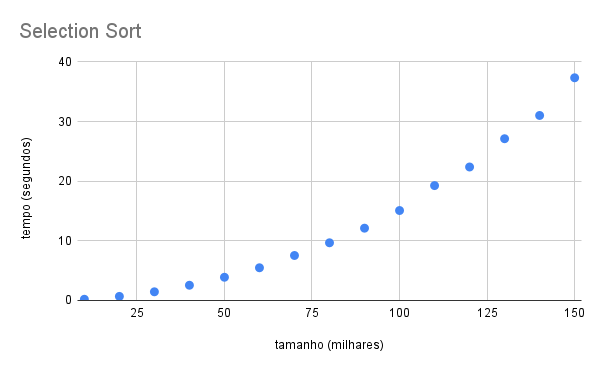
\includegraphics[width=\textwidth]{imagens/SelectionSort1.png}
  \end{figure}

  Podemos testar que se trata de fato de uma parábola poltando os mesmo valores em um gráfico em que ambos os eixos estão em escala logarítmica.
  Se a função tiver o formato $T(n) = an^2$, como nossa análise sugere, ao aplicar o $log$ nos dois lados, temos que:
  \begin{displaymath}
  log(T(n)) = log(an^2) = 2(log(n) + log(a)) = 2log(n) + 2log(a)
  \end{displaymath}
  
  Assim, o que obtemos é a equação de uma reta com inclinação $2$.
  Na Figura \ref{} observamos que de fato em uma gráfico log-log o que obtemos é uma reta com inclinação $1,94$, valor bem próximo do esperado.

  \begin{figure}
    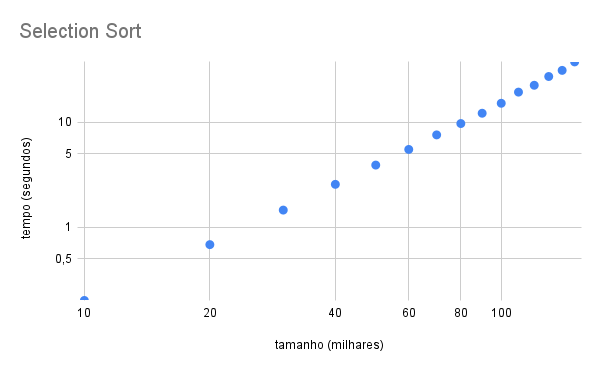
\includegraphics[width=\textwidth]{imagens/SelectionSort2.png}
  \end{figure}

  
  \section{Insertion Sort}

  Nosso segundo algoritmo segue uma ideia também simples.
  Ele ordena uma sequência de maneira análoga a forma como muitas pessoas ordenam cartas de baralhos nas mãos.

  A princípio as cartas estão todas viradas para baixo.
  Elas são inseridas uma por uma na mão do jogador cada qual em sua posição relativa correta.

   \begin{codebox}
     \Procname{$\proc{InsertionSort}(A)$}
     \li \For $j \gets 2$ até $n$
     \li $chave \gets a_j$
     \li    \For $i \gets j-1$ até $1$
     \li    \Do $a_{i+1} \gets a_i$
     \li       \If $a_i > chave$
     \li       \Then sai do laço
               \End
            \End
     \li    $a_{i+1} \gets chave$
     \End
   \end{codebox}

   Para provar a correção deste algoritmo, note que a seguinte propriedade é invariante na linha 2:

   \begin{center}
     a sequência $a_1, \dots, a_{j-1}$ está em ordem crescente
   \end{center}

   A análise do consumo de tempo é similar à do SelectionSort.
   Uma diferença está no fato de que independente da entrada, o SelectionSort sempre processa todos elementos já o InsertionSort pode sair do laço interno precocemente.
   Note então que, quando o pior caso ocorre quando os elementos originalmente estão em ordem descrescente.
   Neste caso, a análise do consumo de tempo é idêntica à do SelectionSort:

   \begin{displaymath}
     T(n) = n + (n-1) + (n-2) + \dots + 2 = \sum_{i=2}^n = \frac{n(n+1)}{2} - 1 \in \Theta(n^2)
   \end{displaymath}

   Assim, no pior caso os algoritmos são identícos.
   Veremos como analisar o caso médio na seção sobre o QuickSort, por ora basta dizer que ela também é $\Theta(n^2)$ neste caso, porém a constante multiplicadora é menor.
   Isso fica evidente quando verificamos o modelo.
   Plotando o tempo e processamento dos dois algoritmos que vimos até aqui em um mesmo gráfico com escala log nos dois eixos, vemos que ambos apresentamos uma reta praticamente com a mesma inclinação -- o primeiro tinha inclinação 1,94 e este 1,88.
   A diferença é no fato de deslocamento vertical que indica uma diferença no fator multiplicador do termo dominante.
   Essa diferença é significativa porque testamos o algoritmo com uma entrada aleatória e, nesse caso, o InsertionSort é um pouco mais eficiente:

   
  \begin{figure}
    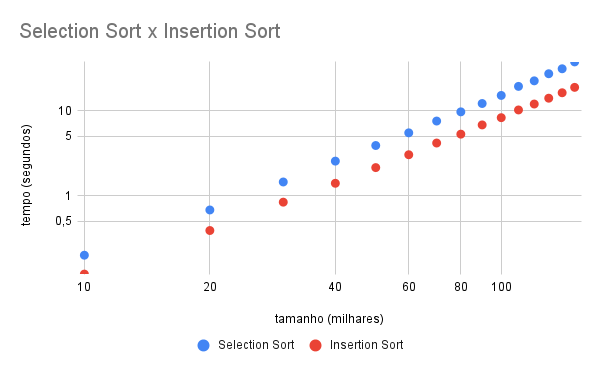
\includegraphics[width=\textwidth]{imagens/SelectionInsertion.png}
  \end{figure}   
  
\section{Merge Sort}

Antes de apresentar o próximo algoritmo, estudaremos um paradigma de projeto de algoritmos chamado {\em divisão-e-conquista} que consiste nos seguintes passos:

\begin{itemize}
  \item {\em Divisão:} a instância original do problema é dividida em um número de instâncias menores.
  \item {\em Conquista:} instâncias suficientemente pequenas são resolvidas diretamente.
    \item {\em Combinação:} se necessário, as soluções das instâncias menores são combinadas em para resolver a instância original.
\end{itemize}

Para exemplificar o paradigma, revisitaremos o algoritmo da busca binária em uma versão recursiva.

\begin{codebox}
  \li \Comment recebe uma sequência ordenada $a_1, \dots, a_n$ e um valor $b$
  \li \Comment devolve V se $b$ está na sequência e F c.c.
  \Procname{$\proc{BuscaBinaria}(A, b)$}
  \li \If $n = 1$
  \li \Then \If $a_1 = b$
  \li \Then \Return V
  \End
  \li \Else
  \li \Return F
  \End 
  \li $m \gets \left \lfloor{\frac{n}{2}}\right\rfloor$
  \li \If $b \leq a_m$
  \li     \Then \Return $BuscaBinaria(A[1:m])$
  \End
  \li \Else \Return $BuscaBinaria(A[m+1:n])$
  \End
\end{codebox}

As linhas 1 a 5 resolvem o caso base ({\em conquista}) enquanto as linhas 6 a 10 dividem o problema em instâncias menores.
Neste caso, não há necessidade de combinar as soluções pois a cada passo, metade da instância original pode ser ignorada.

Para analisar o tempo de processamento deste algoritmo primeiro estabelecemos que as linhas 1 a 5 tomas tempo constante ($c_2$), assim comas as linhas 6, 7 e 9 ($c_1$).
Jás as linhas 8 e 10 são chamadas recursivas.
Assim, o tempo de processamento do pior caso em função do tamanho da entrada $n$ é descrito pela seguinte recorrência:

\begin{eqnarray*}
  T(n) & = & c_1 + T(\left \lceil{\frac{n}{2}}\right \rceil) \\
  T(1) & = & c_2
\end{eqnarray*}

Resolveremos essa recorrência utilizando o método da árvore de recorrência:

% Árvore de recorrência
\begin{center}
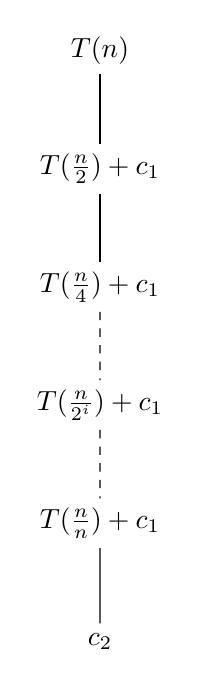
\begin{tikzpicture}
\node {$T(n)$}[sibling distance = 6cm]
child {node {$T(\frac{n}{2}) + c_1$}[sibling distance = 3cm] 
  child {node {$T(\frac{n}{4}) + c_1$}
    child {node {$T(\frac{n}{2^i}) + c_1$} edge from parent [dashed]
      child {node {$T(\frac{n}{n}) + c_1$} 
        child {node {$c_2$} edge from parent [solid]}}}}};
\end{tikzpicture}
\end{center}

A árvore chega no caso base $T(1)$ quando $2^i = n$, ou seja, quando $i = lg(n)$.
Portanto, a altura da árvore é $lg(n)$.
Em cada passo, é somado $c_1$ e no último é somado $c_2$.
Concluímos que:

\begin{displaymath}
  T(n) = c_1.lg(n) + c_2
\end{displaymath}


Talvez um exemplo melhor do paradigma da divisão-e-conquista seja um versão do algoritmo de busca para sequências arbitrárias.
Dividiremos a sequência ao meio, mas neste caso, é preciso buscar nas duas metades dela.
Por fim, precisamos combinar os resultados.
O elemento $b$ está na sequência se ele está na metade direita ou na metade esquerda.

\begin{codebox}
  \li \Comment recebe uma sequência $a_1, \dots, a_n$ e um valor $b$
  \li \Comment devolve V se $b$ está na sequência e F c.c.
  \Procname{$\proc{BuscaRecursiva}(A, b)$}
  \li \If $n = 1$
  \li \Then \If $a_1 = b$
  \li \Then \Return V
  \End
  \li \Else
  \li \Return F
  \End 
  \li $m \gets \left \lfloor{\frac{n}{2}}\right\rfloor$
  \li \Return $BuscaRecursiva(A[1:m])$ ou $BuscaRecursiva(A[m+1:n])$
  \End
\end{codebox}

Como no exemplo anterior, o caso base (linhas 3 a 7) toma tempo constante $c_2$ e as operações de divisão, atribuição e o ou lógico (linhas 8 e 9) também tomam tempo constante $c_2$.
Desta vez, porém, a recursão é aplicada nas duas metades da sequência.
Assim, a recorrência que devemos resolver é:

\begin{eqnarray*}
  T(n) & = & c_1 + T(\left \lceil{\frac{n}{2}}\right \rceil) + T(\left \lfloor{\frac{n}{2}}\right \rfloor)\\
  T(1) & = & c_2
\end{eqnarray*}

Para calcular o resultado dessa recorrência, vamos novamente analisar sua árvore:

% Árvore de recorrência
\begin{center}
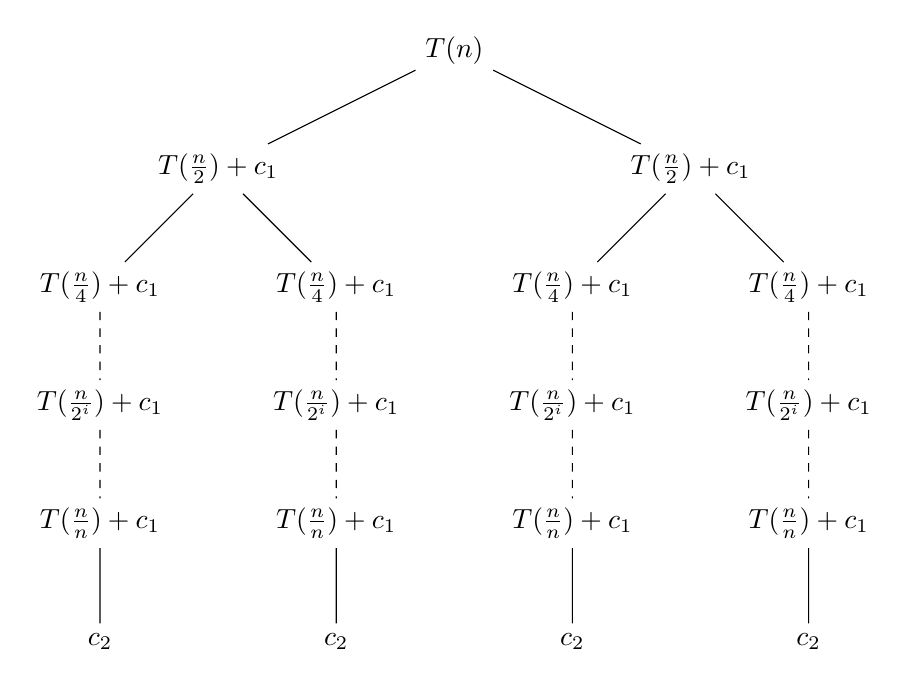
\begin{tikzpicture}
\node {$T(n)$}[sibling distance = 6cm]
child {node {$T(\frac{n}{2}) + c_1$}[sibling distance = 3cm]
  child {node {$T(\frac{n}{4}) + c_1$}
    child {node {$T(\frac{n}{2^i}) + c_1$} edge from parent [dashed]
      child {node {$T(\frac{n}{n}) + c_1$} 
        child {node {$c_2$} edge from parent [solid]}}}}
  child {node {$T(\frac{n}{4}) + c_1$}
    child {node {$T(\frac{n}{2^i}) + c_1$} edge from parent [dashed]
      child {node {$T(\frac{n}{n}) + c_1$} 
        child {node {$c_2$} edge from parent [solid]}}}}}
child {node {$T(\frac{n}{2}) + c_1$}[sibling distance = 3cm] 
  child {node {$T(\frac{n}{4}) + c_1$}
    child {node {$T(\frac{n}{2^i}) + c_1$} edge from parent [dashed]
      child {node {$T(\frac{n}{n}) + c_1$} 
        child {node {$c_2$} edge from parent [solid]}}}}
  child {node {$T(\frac{n}{4}) + c_1$}
    child {node {$T(\frac{n}{2^i}) + c_1$} edge from parent [dashed]
      child {node {$T(\frac{n}{n}) + c_1$} 
        child {node {$c_2$} edge from parent [solid]}}}}};
\end{tikzpicture}
\end{center}

Como no caso anterior, essa árvore chega às folhas quando $2^i = n$, ou seja, quando $i = lg(n)$.
Portanto, a altura dela é $lg(n)$.
Em cada nível dessa árvore dobramos a quantidade de $c_1$ somadas.
Assim, no i-ésimo nível são somados $2^i$ constantes e no último são somados $2^{lg(n)} = n$ constantes.
Portanto, o resultado de nossa recorrência é:

\begin{eqnarray*}
  T(n) & = & c_1.\sum_{i=1}^{lg(n)}2^i + c_2.n\\
  & = & c_1.\frac{1 - 2^{lg(n)}}{1-2} + c_2.n \\
  & = & c_1.(n-1) + c_2.n \\
  & = & (c_1 + c_2).n - c_1 \\
  & \in & \Theta(n)
\end{eqnarray*}

O merge sort, ou algoritmo de ordenação por intercalação, também segue o paradigma da divisão-e-conquista.
A ideia é quebrar a instância original ao meio até que ela tenha apenas um elemento.
Neste caso, o caso base, não é preciso fazer nada pois qualquer sequência com um único elemento está trivialmente ordenada.
O segredo está na combinação das instâncias menores para resolver a instância original.
Para este passo, usaremos um algoritmo de intercalação.

Podemos enunciar o problema da intercalação da seguinte forma:


{\bf Problema da busca}\\

{\bf Entrada:} Duas sequências $a_1, \dots, a_n$ e $b_1, \dots, b_m$ ambas em ordem crescente.

{\bf Saída:} Uma sequência $c_1, \dots, c_{m+n}$ em ordem crescente cujos elementos são os mesmos das sequências da entrada.

Para resolver esse problema utilizamos o seguinte algoritmo:

\begin{codebox}
  \Procname{$\proc{Merge}(A, B)$}
  \li $i \gets 1$
  \li $j \gets 1$
  \li \For $k \gets 1$ até $n+m$
  \li \Do \If ($a_i \leq b_j$ e $i \leq n$) ou $j > m$
  \li \Then $c_k \gets a_i$
  \li $i \gets i + 1$
  \li \Else
  \li $c_k \gets b_j$
  \li $j \gets j + 1$
  \End
  \End
  \li \Return $C$
\end{codebox}

Com isso, podemos escrever o algoritmo de ordenação da seguinte forma:

\begin{codebox}
  \Procname{$\proc{MergeSort}(A, B)$}
  \li \If $n > 1$
  \li \Then  $m \gets \left \lfloor{\frac{n}{2}}\right\rfloor$
  \li $MergeSort(A[1:m])$
  \li $MergeSort(A[m+1:n])$
  \li $A \gets Merge(A[1:m], A[m+1:n])$
\end{codebox}

O caso base do algoritmo ocorre quando $n = 1$.
Neste caso, nada precisa ser feito e o tempo tomado é constante $c$.
Já a linha 4 toma tempo linear no tamanho da entrada $n$.
Com isso, temos que o tempo de execução do algoritmo em função de $n$ é:

\begin{eqnarray*}
  T(n) & = & c_1.n + T(\left \lfloor{\frac{n}{2}}\right\rfloor) + T(\left \lceil{\frac{n}{2}}\right\rceil)\\
  T(1) & = & c_2
\end{eqnarray*}

Analisaremos, então a seguinte árvore de recorrência:

% Árvore de recorrência
\begin{center}
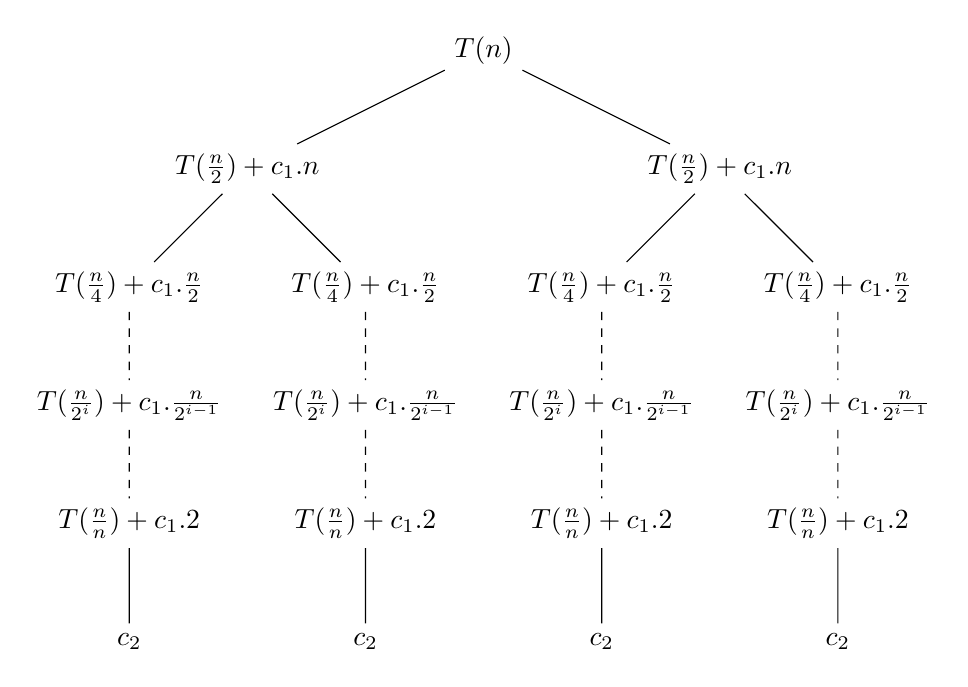
\begin{tikzpicture}
\node {$T(n)$}[sibling distance = 6cm]
child {node {$T(\frac{n}{2}) + c_1.n$}[sibling distance = 3cm]
  child {node {$T(\frac{n}{4}) + c_1.\frac{n}{2}$}
    child {node {$T(\frac{n}{2^i}) + c_1.\frac{n}{2^{i-1}}$} edge from parent [dashed]
      child {node {$T(\frac{n}{n}) + c_1.2$} 
        child {node {$c_2$} edge from parent [solid]}}}}
  child {node {$T(\frac{n}{4}) + c_1.\frac{n}{2}$}
    child {node {$T(\frac{n}{2^i}) + c_1.\frac{n}{2^{i-1}}$} edge from parent [dashed]
      child {node {$T(\frac{n}{n}) + c_1.2$} 
        child {node {$c_2$} edge from parent [solid]}}}}}
child {node {$T(\frac{n}{2}) + c_1.n$}[sibling distance = 3cm] 
  child {node {$T(\frac{n}{4}) + c_1.\frac{n}{2}$}
    child {node {$T(\frac{n}{2^i}) + c_1.\frac{n}{2^{i-1}}$} edge from parent [dashed]
      child {node {$T(\frac{n}{n}) + c_1.2$} 
        child {node {$c_2$} edge from parent [solid]}}}}
  child {node {$T(\frac{n}{4}) + c_1.\frac{n}{2}$}
    child {node {$T(\frac{n}{2^i}) + c_1.\frac{n}{2^{i-1}}$} edge from parent [dashed]
      child {node {$T(\frac{n}{n}) + c_1.2$} 
        child {node {$c_2$} edge from parent [solid]}}}}};
\end{tikzpicture}
\end{center}

Em cada nível da árvore, é somado $2.c_1.n$.
Como a altura dessa árvore também é $lg(n)$ temos que:
\begin{displaymath}
  T(n) = 2.c_1.n.lg(n) + 2.n.c_2 \in \Theta(n.lg(n))
\end{displaymath}

Agora que vimos como resolver três recorrências diferentes usando o método da árvore de recorrência, apresentaremos um resultado geral para resolver recorrências:

\begin{theorem}[Mestre]
  Sejam $a \geq 1$, $b > 1$ e $T(n) = aT(\frac{n}{b}) + f(n)$, então:
  \begin{enumerate}
  \item se $f(n) \in O(n^{log_b(a - \epsilon)})$ para algum $\epsilon > 0$ então $T(n) \in \Theta(n^{log_ba})$
  \item se $f(n) \in \Theta(n^{log_ba})$ então $T(n) \in \Theta(n^{log_ba}lg(n))$
  \item se $f(n) \in O(n^{log_b(a + \epsilon)})$ para algum $\epsilon > 0$ e se $af(\frac{n}{b}) \leq cf(n)$ para algum $c < 1$ e todo $n$ suficientemente grande então $T(n) \in \Theta(f(n))$
  \end{enumerate}
\end{theorem}

\begin{example}
  Comecemos pela recorrência que acabamos de analisar
  \begin{displaymath}
    T(n) = 2T\left(\frac{n}{2}\right) + cn
  \end{displaymath}

  O primeiro passo é avaliar $n^{log_ba}$ que neste caso é $n^{log_22} = n$.
  Então temos que verificar se $f(n) = cn \in \Theta(n)$.
  Neste caso, isso vale.
  Portante se aplica o caso 2 do teorema e temos que:

  \begin{displaymath}
    T(n) \in \Theta(n^{log_22}.lg(n)) = \Theta(n.lg(n))
  \end{displaymath}
\end{example}

\begin{example}
  Considere a recorrência que obtivemos ao analisar a busca binária:
  \begin{displaymath}
    T(n) = T\left(\frac{n}{2}\right) + c
  \end{displaymath}

  O primeiro passo é avaliar $n^{log_ba}$ que neste caso é $n^{log_21} = n^0 = 1$.
  Então temos que verificar se $f(n) = c \in \Theta(1)$.
  Neste caso, isso vale.
  Portante se aplica o caso 2 do teorema e temos que:

  \begin{displaymath}
    T(n) \in \Theta(n^{log_21}.lg(n)) = \Theta(1.lg(n)) = \Theta(lg(n))
  \end{displaymath}
\end{example}


\begin{example}
  Considere agora a recorrência que obtivemos ao analisar a busca recursiva:
  \begin{displaymath}
    T(n) = 2T\left(\frac{n}{2}\right) + c
  \end{displaymath}

  Primeiro avaliamos $n^{log_22} = n$.
  Então temos que verificar se $f(n) = c \in \Theta(n)$.
  Neste caso, isso não é verdade $c$ cresce mais lentamente do que $n$.
  
  Se  $\epsilon = 1$ temos que $n^{log_2(2-1)} = n^0 = 1$ e $c \in O(1)$.
  Portanto podemos aplicar o caso 1 do teorema e temos que:

  \begin{displaymath}
    T(n) \in \Theta(n^{log_22} = \Theta(n^1) = \Theta(n)
  \end{displaymath}
\end{example}

\begin{example}
  Para terminar, considera a seguinte recorrência:
  \begin{displaymath}
    T(n) = 2T\left(\frac{n}{2}\right) + n^2
  \end{displaymath}

  Primeiro avaliamos $n^{log_22} = n$.
  Então temos que verificar se $f(n) = n^2 \in \Theta(n)$.
  Neste caso, isso não é verdade $n²$ cresce mais rapidamente do que $n$.
  
  Se $\epsilon = 2$ temos que $n^{log_2(2+2)} = n^2$ e $n^2 \in \Omega(n^2)$ e $2(\frac{n}{2})^2 = \frac{n^2}{2} \leq \frac{1}{2}.n^2$ para todo $n > 0$.  
  Portanto podemos aplicar o caso 3 do teorema e temos que:

  \begin{displaymath}
    T(n) \in \Theta(f(n)) = \Theta(n^2)
  \end{displaymath}
\end{example}



\section{Quick Sort}
\section{Heap Sort}
